
\chapter{State of the Art} \label{ch:state-of-the-art}

\section{Problem 1 - Tactile Perception} \label{sec:lit-rev-problem-1}

In order to model the contact between the \gls{ee}'s tactile sensors, eight different taxonomies are present\cite*{articulated-hands-force-control-and-kinematic-issues} whereas three most common ones are \gls{pwof}, \gls{hf} and the \gls{sf} model as shown in \figref{fig:contact-models}, within the field of robotics\cite[Chapter 37]{handbook-of-robotics}. \medskip

\begin{figure}[h]
	\centering
	\begin{subfigure}[b]{0.3\textwidth}
		\centering
		
\includegraphics[width=\textwidth]{img/placeholder.png}
		\caption{Point contact model without friction.}
		\label{fig:pwof}
	\end{subfigure}
	\hfill
	\begin{subfigure}[b]{0.3\textwidth}
		\centering
		
\includegraphics[width=\textwidth]{img/placeholder.png}
		\caption{Point contact model with friction.}
		\label{fig:hf}
	\end{subfigure}
	\hfill
	\begin{subfigure}[b]{0.3\textwidth}
		\centering
		
\includegraphics[width=\textwidth]{img/placeholder.png}
		\caption{Soft-finger model.}
		\label{fig:sf}
	\end{subfigure}
	   \caption{The three most commonly used contact models.}
	   \label{fig:contact-models}
\end{figure}

% no friction
The \gls{pwof} model, as shown in \figref{fig:pwof}, can only represent forces along with the normal of the object's surface at the point of contact and thus the model does not support surface deformations between the two contacting objects. This model is applied in cases where very little deformation is present along with the contact being slippery\cite[Chapter 38]{handbook-of-robotics}.\medskip

% Hard finger
The \gls{hf} model, as shown in \figref{fig:hf}, is representative when the friction between objects is great enough to be significant, while the contact deformation is small enough to ignore friction moments\cite[Chapter 38]{handbook-of-robotics}. To model the friction acting on the contact point a great number of methods exist, the most common being the Column friction with different modifications depending on the use case\fakecite. \medskip

% Soft finger
The \gls{sf} model, as shown in \figref{fig:sf}, is used to represent scenarios where both friction and surface deformations are great enough to be impactful in the systems behavior. Due to deformations of the finger an additional torsional moment about the contact normal will be present.
\cite[Chapter 38]{handbook-of-robotics}  \medskip


% draw the model as applied in our case

% subcategories of sf models
Based on the contact model categories described above, the most representative is \gls{sf} since these models can provide descriptions of the contact surface topology, and thus enable the solving of the \gls{iep} by deriving surface features for pose estimation. Within the category of \gls{sf} models a method fit for this project's use case is to be chosen to solve problem \ref{prob:1}. \gls{sf} models can furthermore be divided up into three different categories: \gls{aebm}, \gls{efm} and \gls{fem} \cite{a-modified-elastic-foundation-contact-model-for-application-in-3d-models-of-the-prosthetic-knee}. \medskip


% reformulate
% \gls{aebm} are theoretical formulations of elasticity calculating contact areas and stresses on both the surface and the sub-surface of the contacting bodies, but are restricted to simple geometries. The classical Hertz contact model (Hertz, 1882; Johnson, 1995)

% 

% 1) I want to model contacts
% 2) there exist 8 different modeling taxonolies
% 3) three are most common
% 	3.a) explain each of the three 
% 4) since soft supports the behavior we want we choose that one
% 5) what method categories exist within soft finger modelling



% In order to model the pressure distribution in the contact area different models have been devel-
% oped that fall into three main categories: analytical elasticity-based models, elastic foundation models
% (EFM) and finite element models (FEM) (Pérez-González et al., 2008). Analytical models are based on
% theoretical formulations of elasticity calculating contact areas and stresses on both the surface and the
% sub-surface of the contacting bodies, but are restricted to simple geometries. The classical Hertz con-
% tact model (Hertz, 1882; Johnson, 1995) and others derived from it are part of this category. However,
% robotic fingertips are made of nonlinear elastic materials. For that reason, the Hertzian contact model
% does not accurately represent this type of contact. EFMs were developed in order to allow a simple
% discrete contact calculation in more general surface geometries modelling the deformable part of the
% contact as a layer over a rigid base, and a series of discrete and independent springs in the contact
% normal direction. An application of this category of models is presented in Section 3.4 where it is used
% to create a simulation of a general tactile sensor and validated in robot grasping applications. FEMs
% have been increasingly used over recent years given that they supply information about the sub-surface
% stresses and strain in volumetric finite elements. However, they are excessively time consuming for fast
% simulation in dynamic grasping and manipulation models. Therefore, simplified numerical models are
% interesting alternatives.

% with friction



% soft finger


% When choosing a representative contact model, two overarching groups exist: linear and non linear models. While the linear models often are too simple to properly represent the real phenomena, their simplicity often make them a popular choice for practical reasons. \medskip

% Within the linear models group we find the most common model: The Hertzian contact model\cite*{on-the-contact-of-rigid-elastic-solids-and-on-hardness}. This model makes the assumptions that
% the objects consist of linear elastic materials when in contact and the contact deformations are small compared to the dimension of object.


% non-linear models

% When considering the non linear contact models, the simpler 

% The Hertzian contact model specifically assumed linear elastic objects in contact with small deformation. Later, the study of contact mechanics became a branch in mechanics. One of the important results in his seminal paper postulated that where N is the normal force, a is the radius of circular contact area, and C is a proportional constant. Equation (2), derived by Hertz [13], describes the growth of radius of circular contact area as proportional to the normal force raised to the power of 3 1 . It is important to note that Hertz had assumed that ( i ) the contact is linear elastic and ( ii ) the deformation is small.



% 

% \begin{center}
%     \renewcommand{\arraystretch}{1.2}
%     \begin{minipage}{.48\linewidth}
%         \vspace{0pt}
%         \centering
%         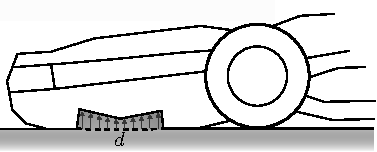
\includegraphics[width=.95\textwidth]{chapters/modeling/fig/measure-displacement.pdf}
%     \end{minipage}%
%     \vspace{15pt}
%     \begin{minipage}[t]{.48\linewidth}
%         \vspace{0pt}
%         \captionsetup{type=figure}
%         \captionof{figure}{The friction forces $\mathbf{f}_f$ and contact model keeps the object $\{O\}$ from slipping between the \gls{ee}'s fingers when the gravitational pull $\mathbf{f}_g$ is acting on it.}
%         \label{fig:measure-displacement}
%     \end{minipage}%
% \end{center}

% in order to perform tactile perception we need to model the contact between the end effector and the object of interest -> 
% 	This model needs to provide descriptions of parameters such as pressure and area for the contact to be 
% 	This model needs to contain the pressure and deformation caused by the contact in order to recreate the surface of contact





% What are contact models and what do they describe?
% For tactile perception it is needed to model the contact between the robotic manipulator finger and the object. The model will here 

% we need a model


%  what do we wish to model contact forces and how they can relate to deformation. Friction to determine how much force to apply in order to keep the object in the grasp.


%  


% flush out what exactly the model i want to use looks like


% When considering different methods for modeling contact interfaces, each can be categorized depending on which parameters the model describe the relation between. This results in the following groupings: contact-area-force models, stress-strain models, force-displacement models and 

% How are models grouped and what groupings exist?

% Contact models can be grouped based on the what parameters the relation is describing.







% Contact Area vs. Applied Force


% Hertzian contact model

% Soft Contact Model (More general Hertzian model)

% Viscoelastic Soft Contact Model.

% 	 Kelvin–Voigt/Maxwell model
% 	  Fung’s model

% Other contact models (research)



% Boussinesq–Cerruti’s

% Love’s solution 




% Love's formulation 




% What is tactile perception? Why is it relevant? \\
% How is a tactile sensor constructed \cite{recent-progress-in-technologies-for-tactile-sensors}
% what different types exist and which one is present in the model provided.


% \textit{"Representations of tactile data are commonly either inspired by machine vision feature descriptors"}

% often used in computer vision context, where each tactile image 

% Addressing the problem 





\section{Problem 2 - Pose Estimation} \label{sec:lit-rev-problem-2}

\section{Problem 3 - In-Hand Manipulation} \label{sec:lit-rev-problem-3}